\documentclass[aps, twocolumn, floatfix, superscriptaddress]{revtex4}
\usepackage{amsmath, amssymb, amsfonts, gensymb}
\bibliographystyle{apsrev}
\usepackage{graphicx}
\graphicspath{ {Figures/} }
\newcommand{\tdc}[3][]{\frac{\mathrm{d}^{#1}#2}{\mathrm{d}#3^{#1}}} % total differential change.
\newcommand{\pdc}[3][]{\frac{\partial^{#1} #2}{\partial #3^{#1}}} % partial differential change.
\newcommand{\td}[1]{\mathrm{d}#1}
\newcommand{\pd}[1]{\partial#1}

\begin{document}

\title{Dynamics of a self-propelled c-boat at the air-water interface}

\author{V. S. Akella}
\affiliation{Collective Interactions Unit, OIST Graduate University, 1919-1 Tancha, Onna-son, Okinawa, Japan 904-0495}
\author{D. K. Singh}
\affiliation{Collective Interactions Unit, OIST Graduate University, 1919-1 Tancha, Onna-son, Okinawa, Japan 904-0495}
\author{S. Mandre}
\affiliation{School of Engineering, Brown University, 182 Hope Street, Providence, RI 02906, USA}
\author{M. M. Bandi}
\affiliation{Collective Interactions Unit, OIST Graduate University, 1919-1 Tancha, Onna-son, Okinawa, Japan 904-0495}
\email[Corresponding Author: ]{bandi@oist.jp}

\date{\today}

\begin{abstract}
In the present work, we report the dynamics of a \emph{c-boat} at the air-water interface. A \emph{c-boat} is a disc-shaped agarose gel tablet with all the water in the agarose gel replaced by camphoric acid. When a c-boat is placed at the air-water interface, it is spontaneously set in motion by the solutal Marangoni forces. Moreover, we observe three different modes of motion, namely harmonic, continuous and periodic when the air-water interfacial tension is modified. We explain these modes in terms of a dimensionless parameter $\xi$. From our experiments, we estimated a critical value $\xi_{c} \simeq 75$ for which the c-boat moves with constant speed. The harmonic, continuous and periodic motions are observed when $\xi > \xi_{c}$,  $\xi \simeq \xi_{c}$ and $\xi < \xi_{c}$ respectively. Experimentally, the parameter $\xi$ is varied by changing the interfacial tension of the air-water interface using Sodium Dodecyl Sulfate (SDS).
\end{abstract}

\maketitle
\section{Introduction}
\section{Experimental Section}
A \emph{c-boat} is a disc shaped agarose gel tablet with the water in the gel matrix replaced by camphoric acid. The method for the preparation of c-boats is described elsewhere (ref to paper 1). In the research work reported in this article, we used c-boats of diameter $3\ \mathrm{mm}$ and thickness $1\ \mathrm{mm}$. When needed, we used Sodium Dodecyl Sulfate (Wako Pure Chemical Industries, Ltd., Cat. No. 196-08675) to modify the air-water interfacial tension. The basic experimental setup consists of a 25 $\mathrm{cm}$ diameter glass petri dish filled with approximately 2 liters of de-ionized water (obtained from Milli-Q Integral Water Purification System with resistivity, $\rho=18.2\ \mathrm{M}\Omega\cdot\mathrm{cm}$ at 25\celsius). The petri dish is illuminated using an LED light tablet from bottom and the motion of the c-boat is recorded with Nikon D800E camera at 30 frames per second from top. The position and the velocity of a c-boat are calculated using an image analysis program written in MATLAB. The air-water interfacial tension measurements are performed using pendant drop method on an OneAttension Theta tensiometer at 25\celsius. 

\section{Results and Discussion}
\subsection{Mechanism of self-propulsion}\label{sec:propmech}
When a c-boat is placed at the air-water interface, camphoric acid molecules are spread radially outwards on to the air-water interface by the interfacial tension forces. However, the spreading can \emph{not} continue forever due to the dissolution of camphoric acid in water which results in radially symmetric camphoric acid concentration gradients around the c-boat. The dissolved camphoric acid molecules decrease the air-water interfacial tension. As a result, there are symmetrical interfacial tension gradients around the c-boat. There is \emph{no} net force acting on the c-boat when the interfacial tension gradients are symmetric. However, the symmetry is spontaneously broken by fluctuations in the temperature or air currents in the surroundings. Once the symmetry is broken, there is a net force acting on the c-boat which causes it to move to a location where the interfacial tension is higher or the camphoric acid concetration is lower. The asymmetry is further enhanced by the motion of c-boat. Note that, the camphoric acid molecules do \emph{not} have any preferential affinity towards interface unlike surfactant molecules which preferentially occupy (below Critical Micelle Concentration) the interface. Therefore the surface activity of camphoric acid molecules is \emph{not} similar to that of surfactant molecules. The motion of c-boat would continue as long as there is camphoric acid in the c-boat. However, during the course of the experiment, the amount of camphoric acid in a c-boat constantly decreases due to dissolution of camphoric acid in water. At any instant of time during the experiment, there exists an outer annulus of the c-boat in which the camphoric acid, lost due to dissolution, is replaced by water. As a consequence of this process, the concentration of camphoric acid at the edge of c-boat is constantly decreasing resulting in weaker interfacial tension gradients and hence decrease in the speed of c-boat as shown in figure~\ref{fig:lifetime}. During the course of the experiment the physical structure of the c-boat (agarose-gel-disc) is intact therefore the viscous drag does not change. Another mechanism for the loss of camphoric acid is: evaporation into the surroundings. However, we found that in case of camphoric acid dissolution is dominant over evaporation. Note that the dissolution of camphoric acid decreases the interfacial tension of water globally however the amount of camphoric acid dissolved from one c-boat ($\simeq 7\ \mathrm{mg}$) is negligibly small to modify the interfacial tension of water globally by a measurable amount. The interfacial tension of water, when saturated with camphoric acid ($\simeq 8\ \mathrm{g/l}$), is $\simeq 60\ \mathrm{dy/cm}$. Figure~\ref{fig:lifetime} shows the speed of c-boat as function of time fitted to an exponential decay in time. The decay constant, $\tau \simeq 40\ \mathrm{min}$ is interpreted as the life time of the c-boat. \par
\begin{figure}[h]
    \begin{center}
       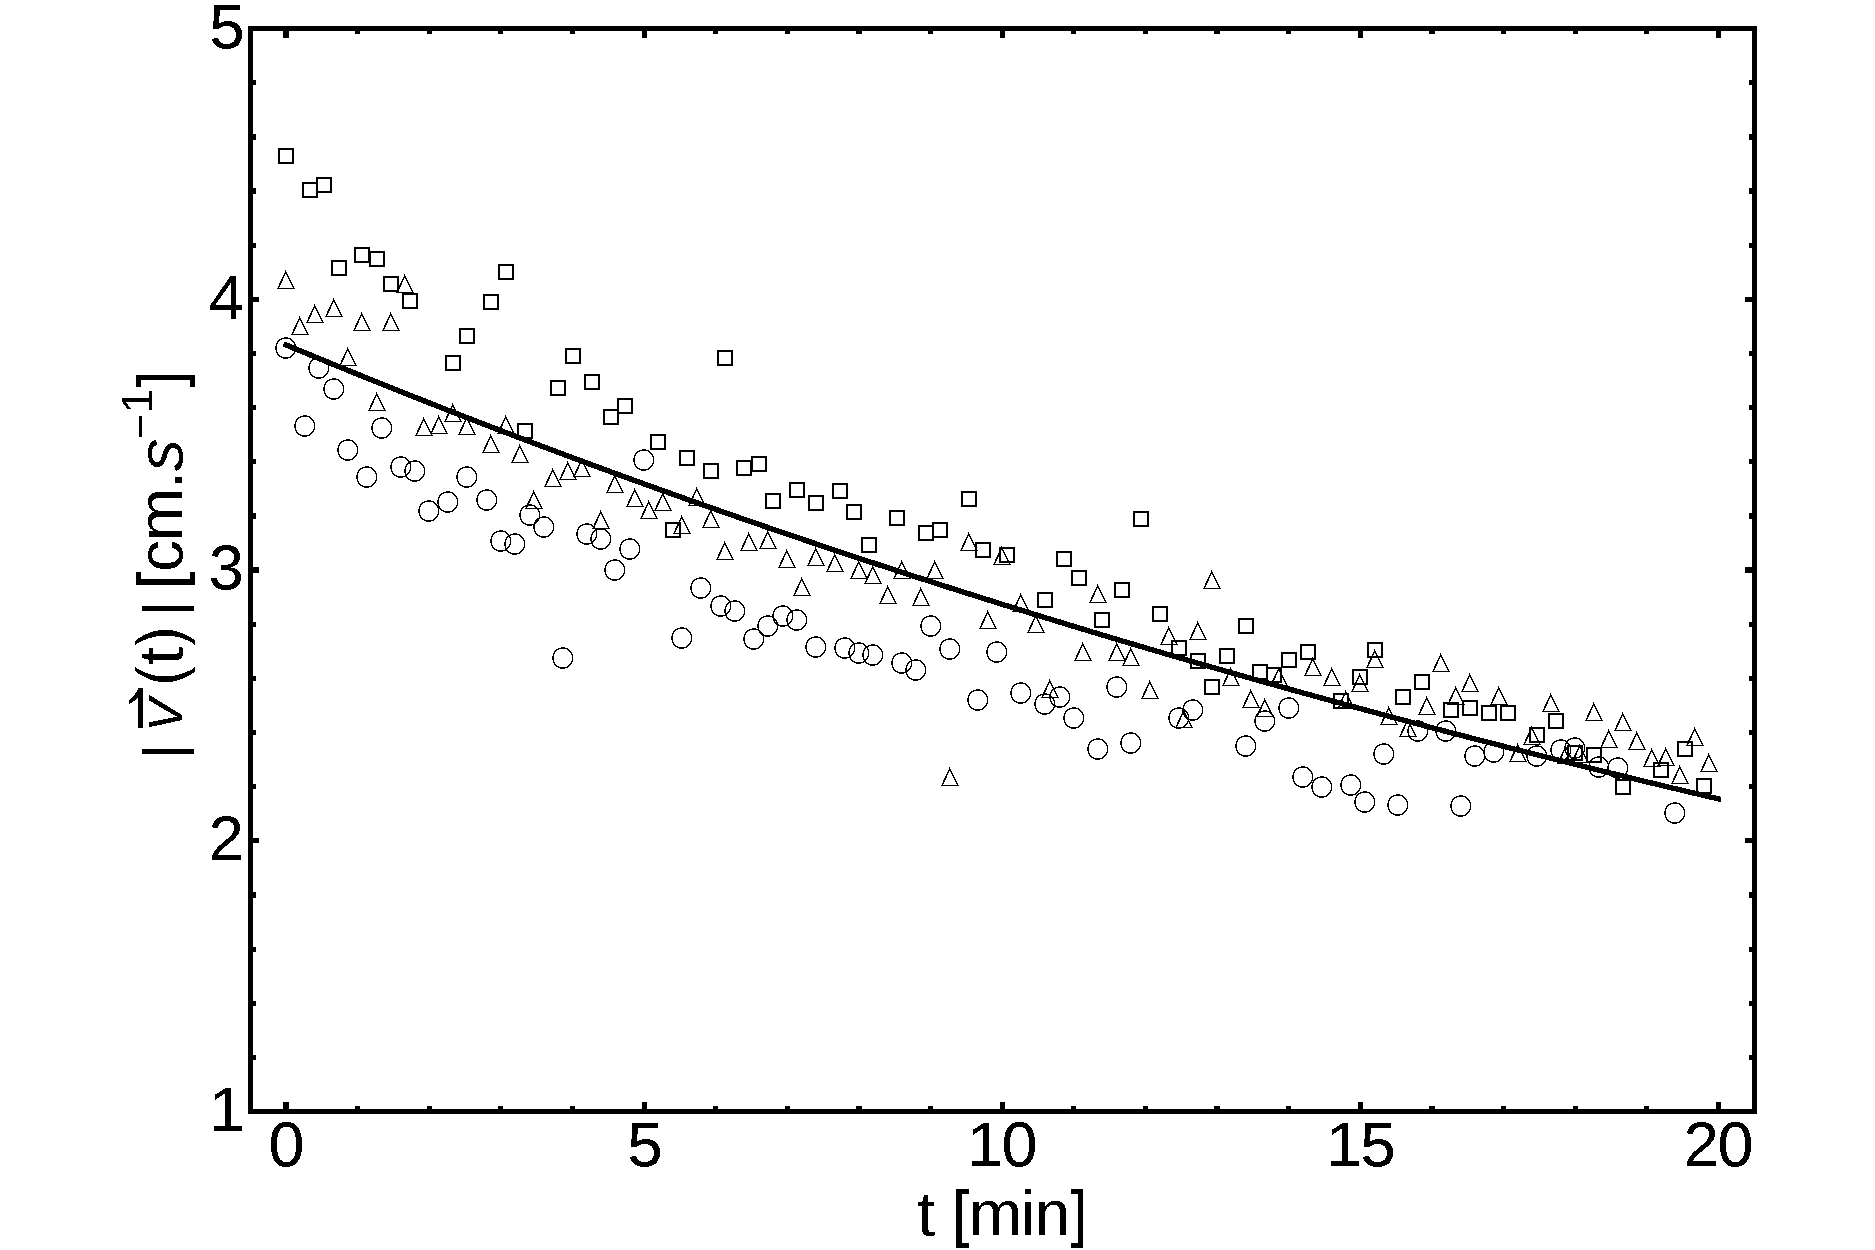
\includegraphics[scale=0.25]{figure6.pdf}
    \end{center}
    \caption{Lifetime of the c-boat.}
    \label{fig:lifetime}
\end{figure}
\subsection{Oscillatory Motion of the C-boat}
\label{sec:oscboat}
Another interesting phenomenon observed in c-boat dynamics is the oscillatory motion. Figure~\ref{fig:uvst_72dypcm} shows the time traces of the c-boat speed at different intervals during the course of experiment. Note that the average speed at different intervals decreases due to the dissolution of camphoric acid in water (refer section~\ref{sec:propmech}). The oscillations arise due to the competition between the Marangoni forces and the viscous forces. The Marangoni forces accelerate the c-boat to larger speed $U_{B}$, however the viscous forces which scale as $U_{B}^{2}$ retard the motion of c-boat. As the c-boat slows down, the Marangoni forces again acclerate the c-boat. This driving and damping cycle results in oscillations in the speed of c-boat. When there is a balance between the driving and damping forces the c-boat moves with constant speed, as shown in figure~\ref{fig:uvst_72dypcm}c. During the course of the experiment, the amplitude of oscillations decreases and the period of oscillation increses (experimental verification in later section). \par
\begin{figure}[h!]
    \centering
	\begin{minipage}[c]{0.45\linewidth}
		\centering
		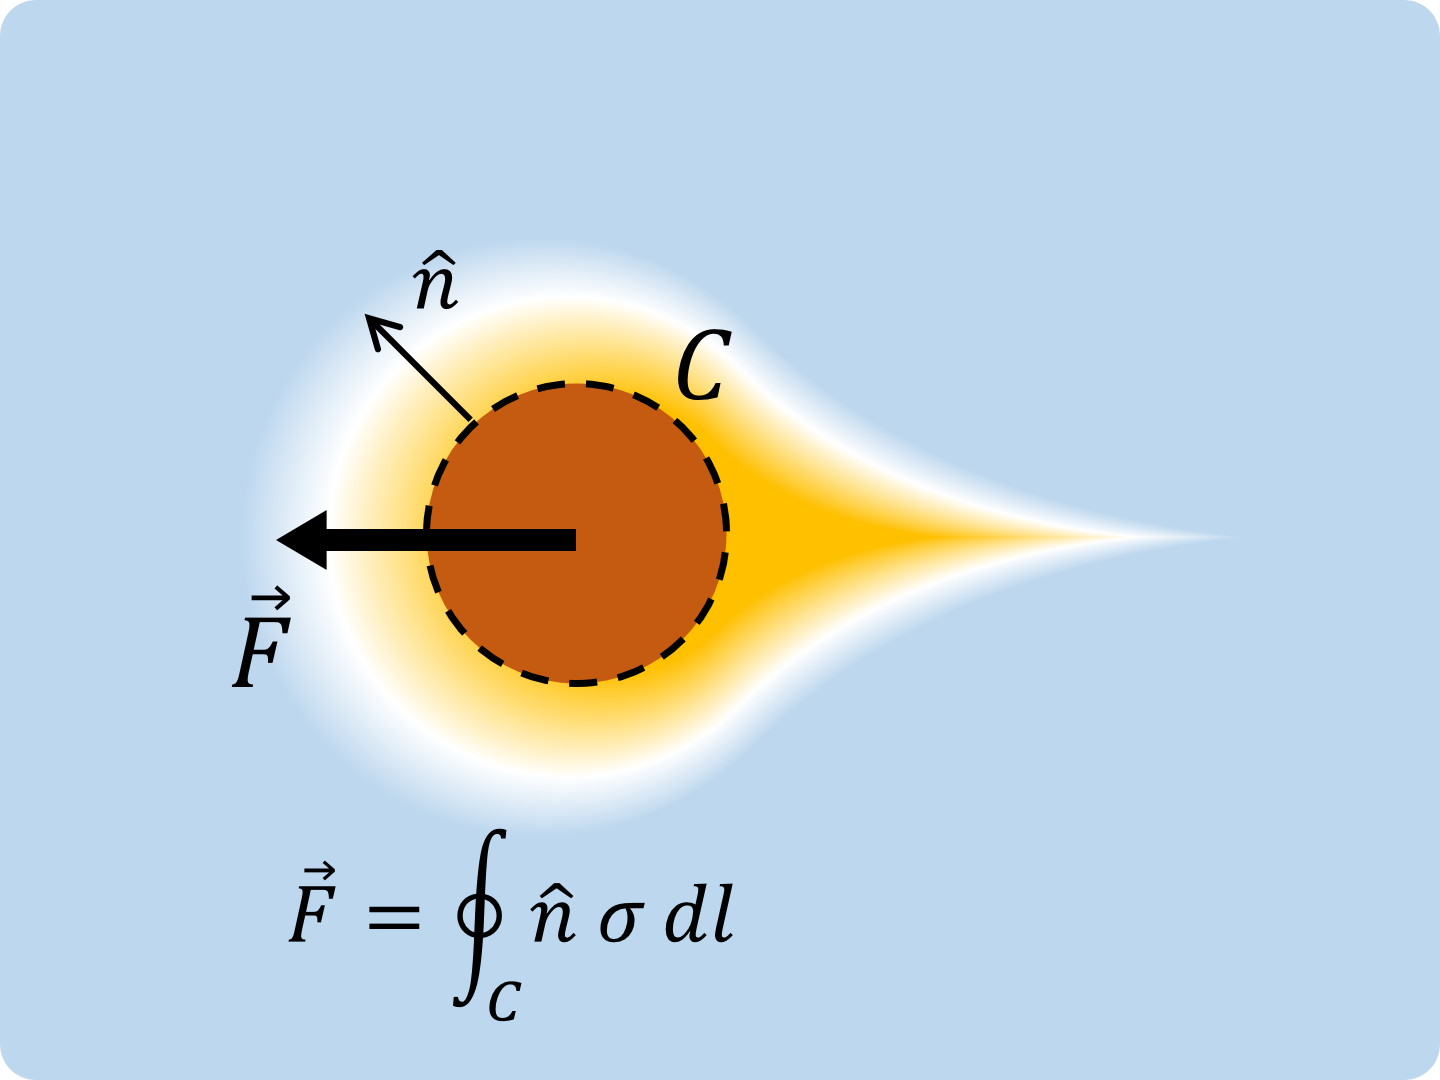
\includegraphics[width=\textwidth]{figure2_v2.png}
		% \caption{Top view}\label{fig:schem_top}		
	\end{minipage}\hspace{0.25cm}
	\begin{minipage}[c]{0.45\linewidth}
		\centering
		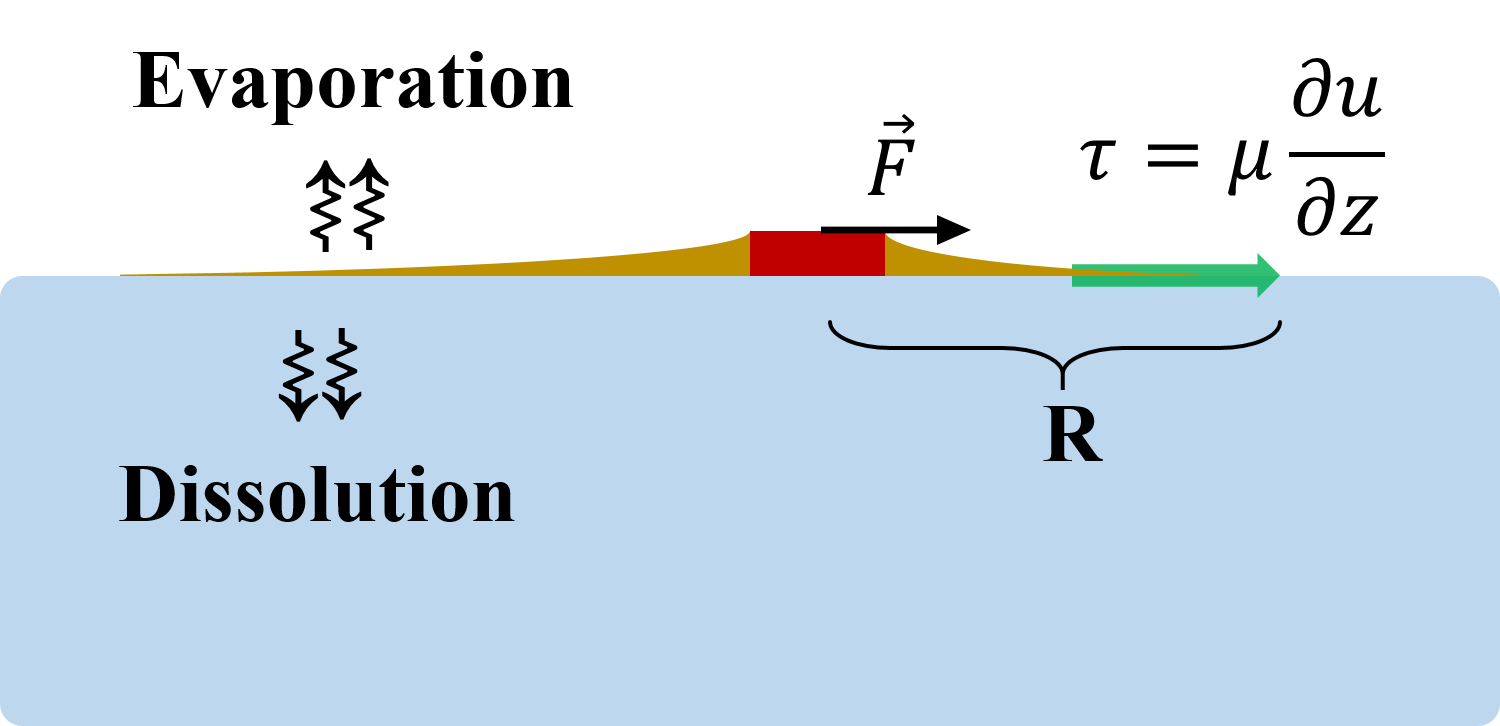
\includegraphics[width=\textwidth]{figure3_v2.png}
		% \caption{Side view}\label{fig:schem_side}
	\end{minipage}
	\caption{Schematic of c-boat in motion (a) top view (b) side view. Viscous drag \emph{not} shown in schematic.}\label{fig:schematic}
\end{figure}
The equation of motion of c-boat at the air-water interface is given by:
\begin{equation}\label{eq:eomgeneral}
\begin{aligned}
m \tdc{\mathbf{u}_{B}}{t} &= -\mathbf{F}_{D} + \oint_{C} \sigma \ \hat{\mathbf{n}} \ \td{l} \\
\mathbf{F}_{D} &\sim \rho\ a^{2} \left|\mathbf{u}_{B}\right|^{2} \hat{\mathbf{u}}_{B}
\end{aligned}
\end{equation}
where, $\mathbf{F}_{D}$ is the viscous drag acting on the c-boat. 
\subsubsection{Estimation of c-boat velocity scale}
For brevity, let us assume that the c-boat exhibits rectilinear motion then the set of equations~\ref{eq:eomgeneral} simplifies to
\begin{equation}
m \tdc{u_{B}}{t} \simeq -\rho\ a^{2}\ u_{B}^{2} + \Delta\sigma\ a
\end{equation}
where, $\Delta\sigma$ is the interfacial tension difference experienced by the c-boat due to the variation in camphoric acid concentration in forward and backward directions of the c-boat. We can obtain a scaling for the average speed, $U_{B}$ of the c-boat as, 
\begin{align}
0 &\simeq -\rho\ a^{2}\ U_{B}^{2} + \Delta\sigma\ a  \nonumber \\
\implies U_{B} &\simeq \sqrt{\frac{\Delta\sigma}{\rho a}} 
\end{align}
\subsubsection{Estimation of Marangoni velocity scale}
The shear stress caused by the interfacial tension gradients is balanced by the viscous stress (figure~\ref{fig:schematic}b).
\begin{align*}
\tau &= \mu \pdc{u_{M}}{z} \\
\implies \pdc{\sigma}{x} &= \mu \pdc{u_{M}}{z} \\
\end{align*} 
where, $u_{M}$ is the fluid velocity at the air-water interface. The Marangoni velocity scale, $U_{M}$ is given by
\begin{equation*}
U_{M} \simeq \frac{\Delta\sigma\ \delta}{\mu R}
\end{equation*}
where, $\delta \sim \sqrt{\frac{\nu R}{U_{M}}}$ is the boundary layer thickness. Substituting $\delta$ yields, 
\begin{equation}
U_{M} = \sqrt[3]{\frac{\Delta\sigma^{2}}{\rho \mu R}}
\end{equation}
\subsubsection{Dimensionless parameter, $\xi$}
The distance from the center of c-boat at which camphoric acid molecules, moving at speed $U_{M}$, are overtaken by the c-boat, moving at speed $U_{B}$, can be obtained by equating the speeds $U_{B}$ and $U_{M}$ and is given by
\begin{equation}\label{eq:rubequm}
R = \sqrt{\frac{\Delta\sigma\rho}{\mu^{2}}}\ a^{3/2}
\end{equation}
From equation~\ref{eq:rubequm}, we define a dimensionless parameter $\xi$ as
\begin{equation}
\xi = \frac{R}{a} = \sqrt{\frac{\Delta\sigma\rho\ a}{\mu^{2}}}
\end{equation}
We \emph{define} a critical value $\xi_{c}$ for the parameter $\xi$ at which the c-boat moves with constant speed. The critical value $\xi_{c} \simeq 75$ is estimated from the experimental data in figure~\ref{fig:uvst_72dypcm}c. \par
Naturally, the dimensionless parameter, $\xi$ constantly decreases during the expriment due to the dissolution of camphoric acid in water. However, we varied $\xi$ by modifying the air-water interfacial tension of water using SDS. Figure~\ref{fig:uvst_65dypcm} shows the speed traces of a c-boat at different intervals of time when the air-water interfacial tension is decreased to $65\ \text{dy/cm}$. We observe that, the average speed of the c-boat at different intervals decreases and the period of the oscillations increases. Another subtle observation is the distance travelled by the c-boat between oscillations is approximately equals to the distance, $\lambda$ out to which camphoric acid molecules are spread by the Marangoni flow before the dissolution occurs. During the course of experiment $\lambda$ constantly decreases due to dissolution of camphoric acid in water. 
\begin{figure*}[h!]\label{fig:uvst_72dypcm}
    \centering
	\begin{minipage}[c]{0.3\linewidth}
		\centering
		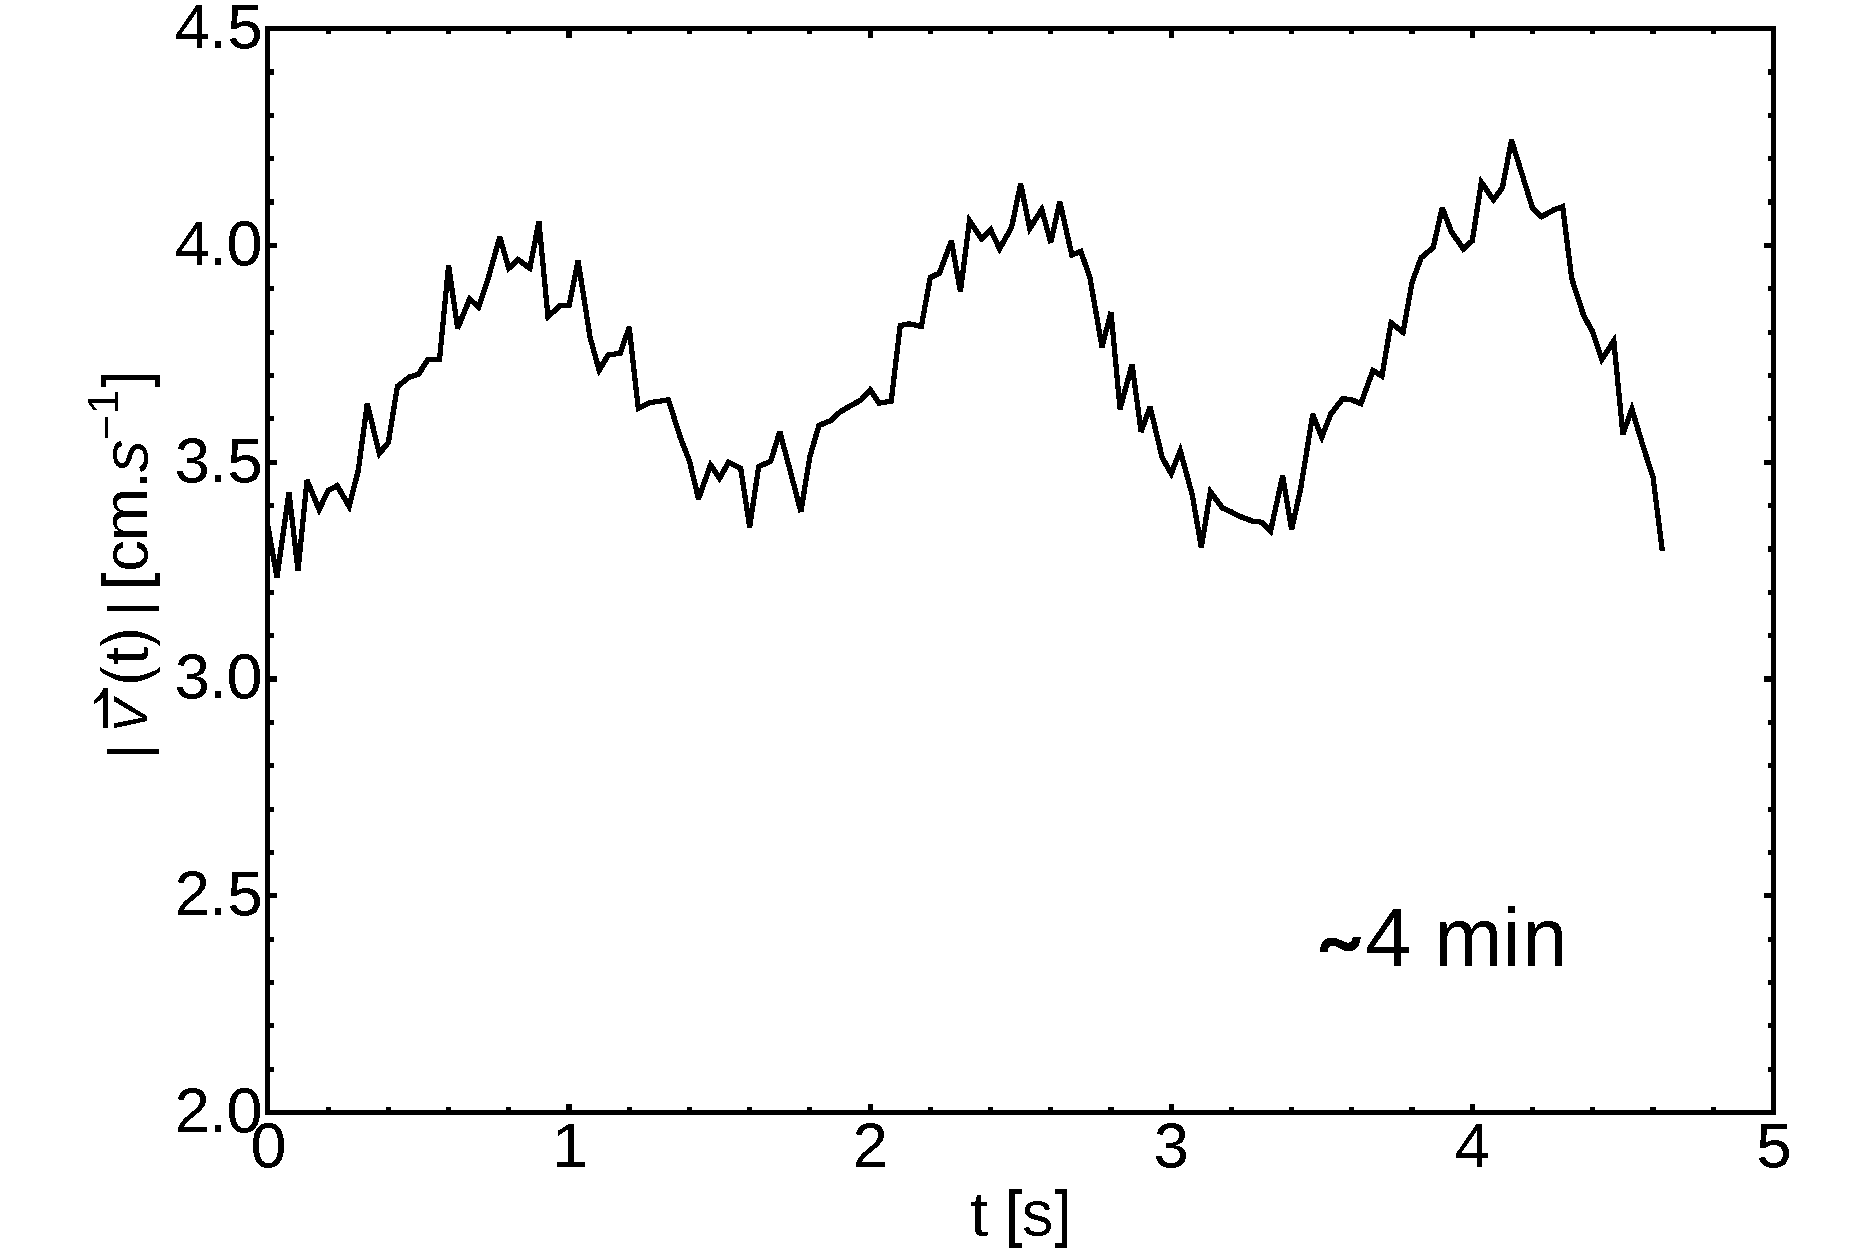
\includegraphics[width=\textwidth]{uvst_72dypcm_a.pdf}
		% \caption{$\xi > \xi_{c}$}\label{fig:uvst_72dypcm_a}		
	\end{minipage}
	\begin{minipage}[c]{0.3\linewidth}
		\centering
		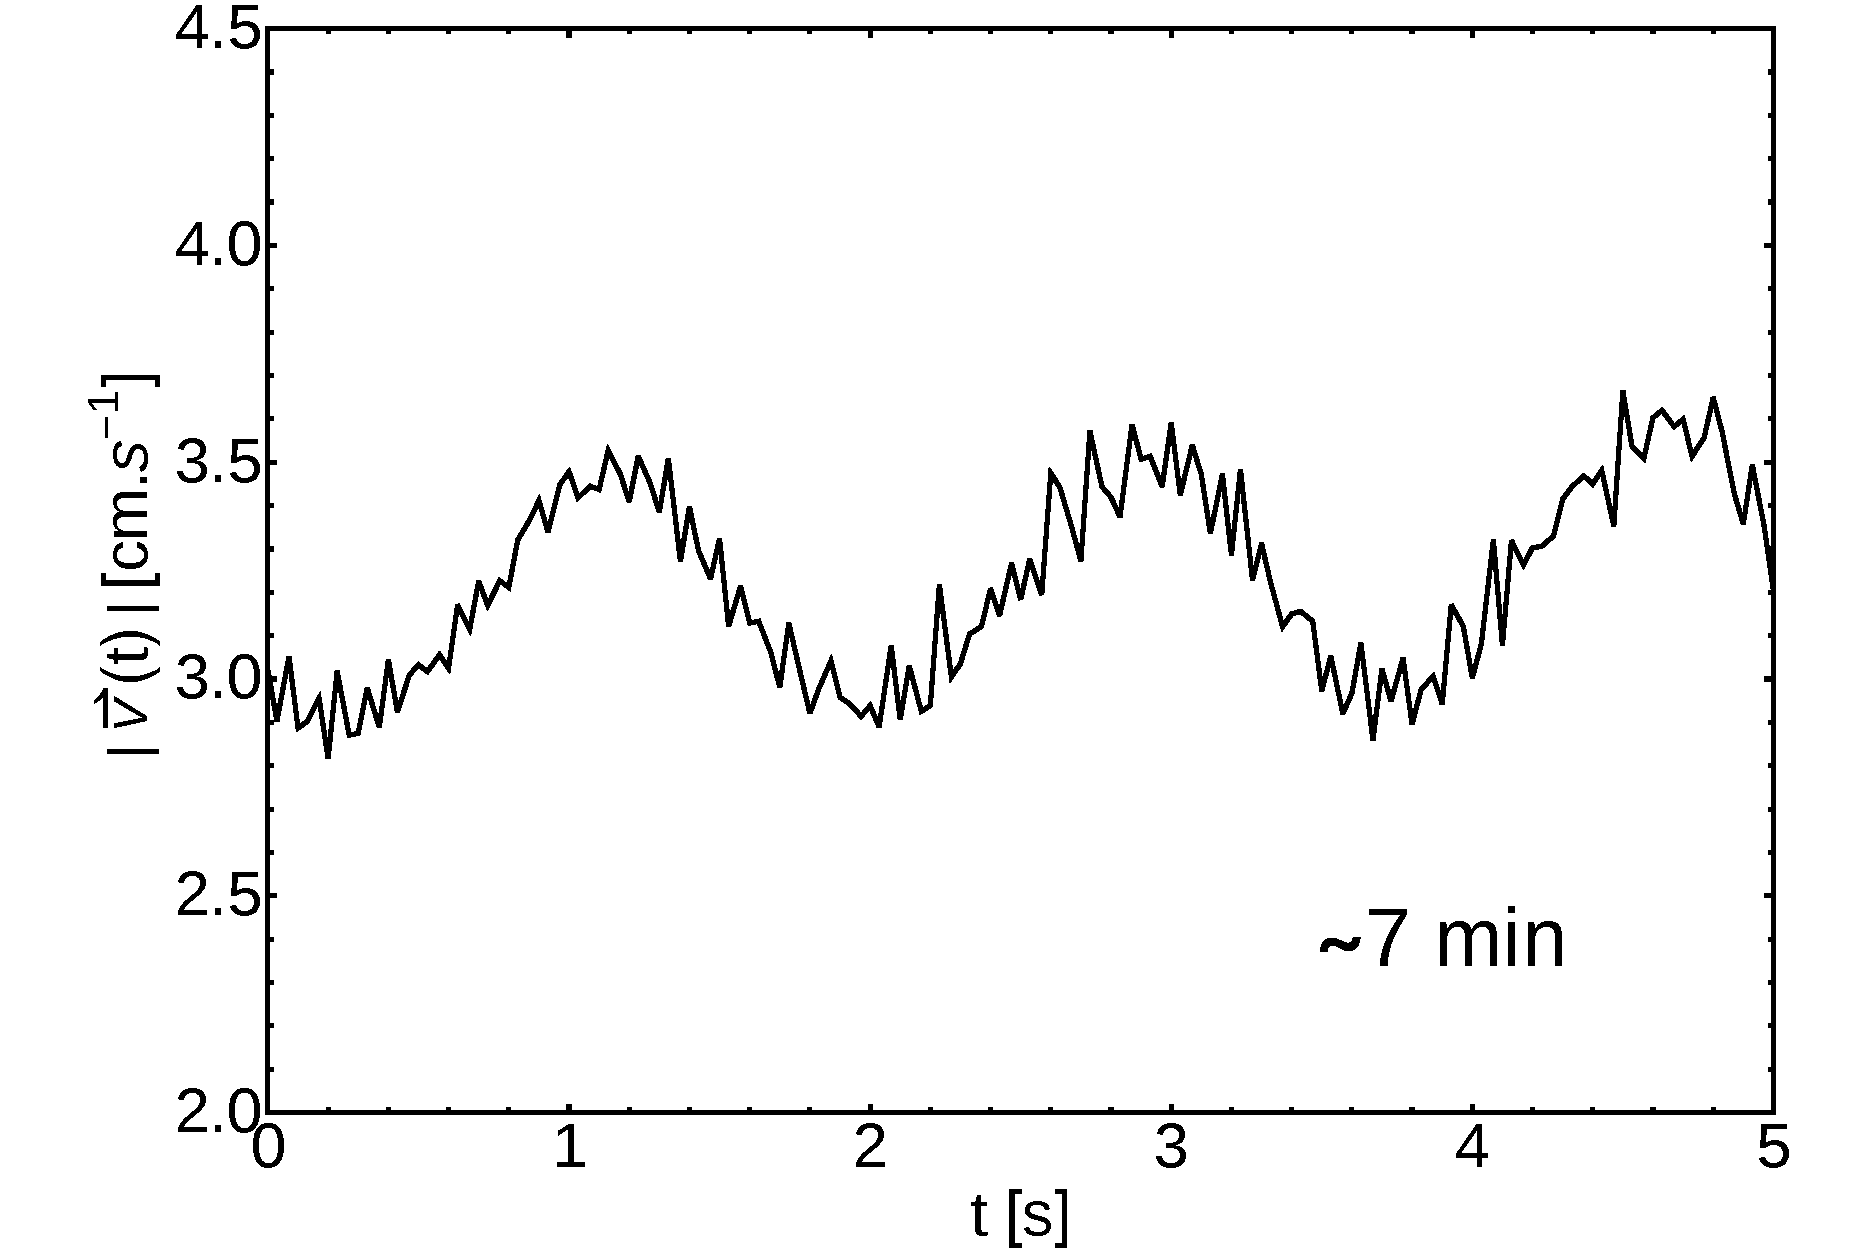
\includegraphics[width=\textwidth]{uvst_72dypcm_b.pdf}
		% \caption{$\xi > \xi_{c}$}\label{fig:uvst_72dypcm_b}
	\end{minipage}
	\begin{minipage}[c]{0.3\linewidth}
		\centering
		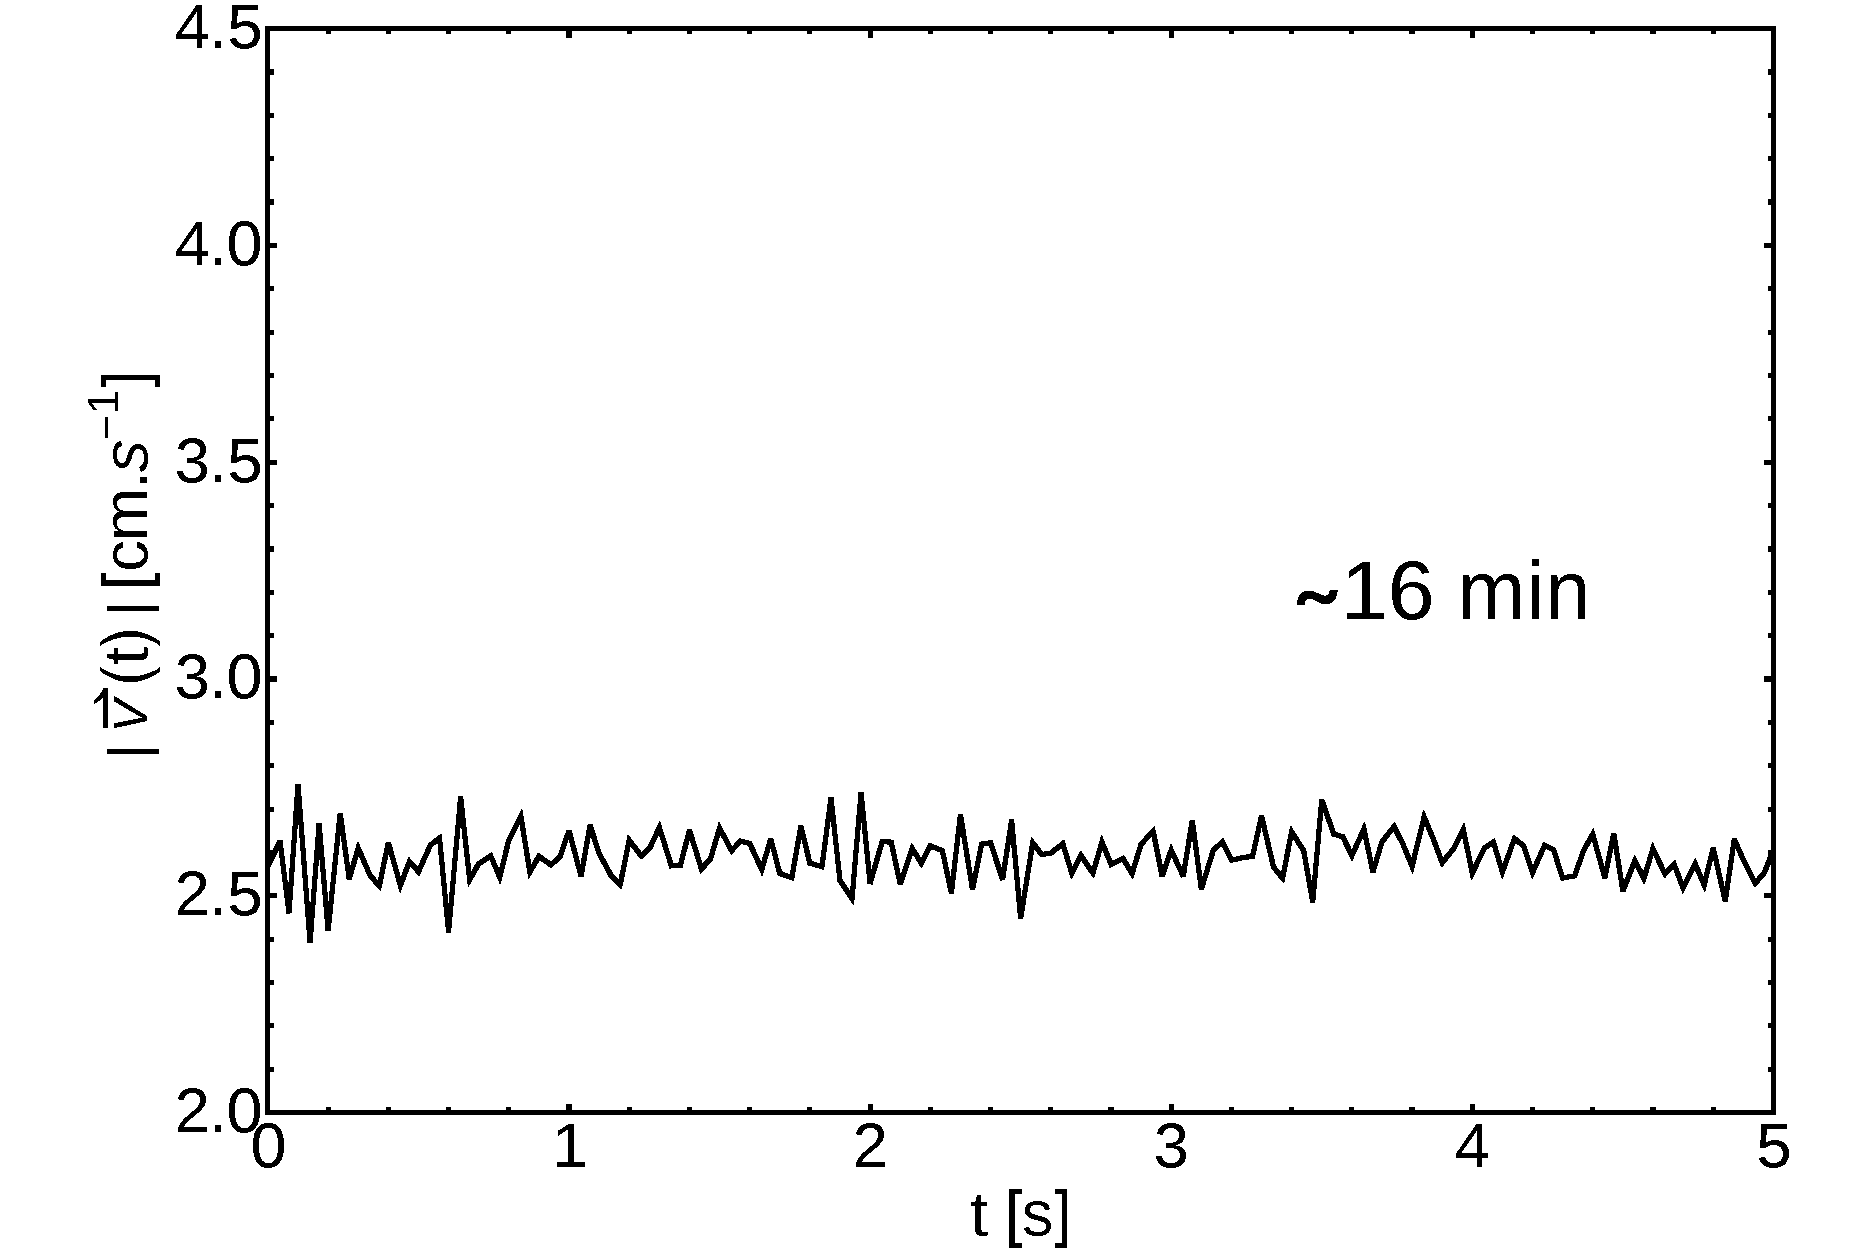
\includegraphics[width=\textwidth]{uvst_72dypcm_c.pdf}
		% \caption{$\xi \simeq \xi_{c}$}\label{fig:uvst_72dypcm_c}
	\end{minipage}
	\caption{$\xi > \xi_{c}$, $\xi > \xi_{c}$ and $\xi \simeq \xi_{c}$}\label{fig:uvst_72dypcm}
\end{figure*}
\begin{figure*}[h!]
    \centering
	\begin{minipage}[c]{0.3\linewidth}
		\centering
		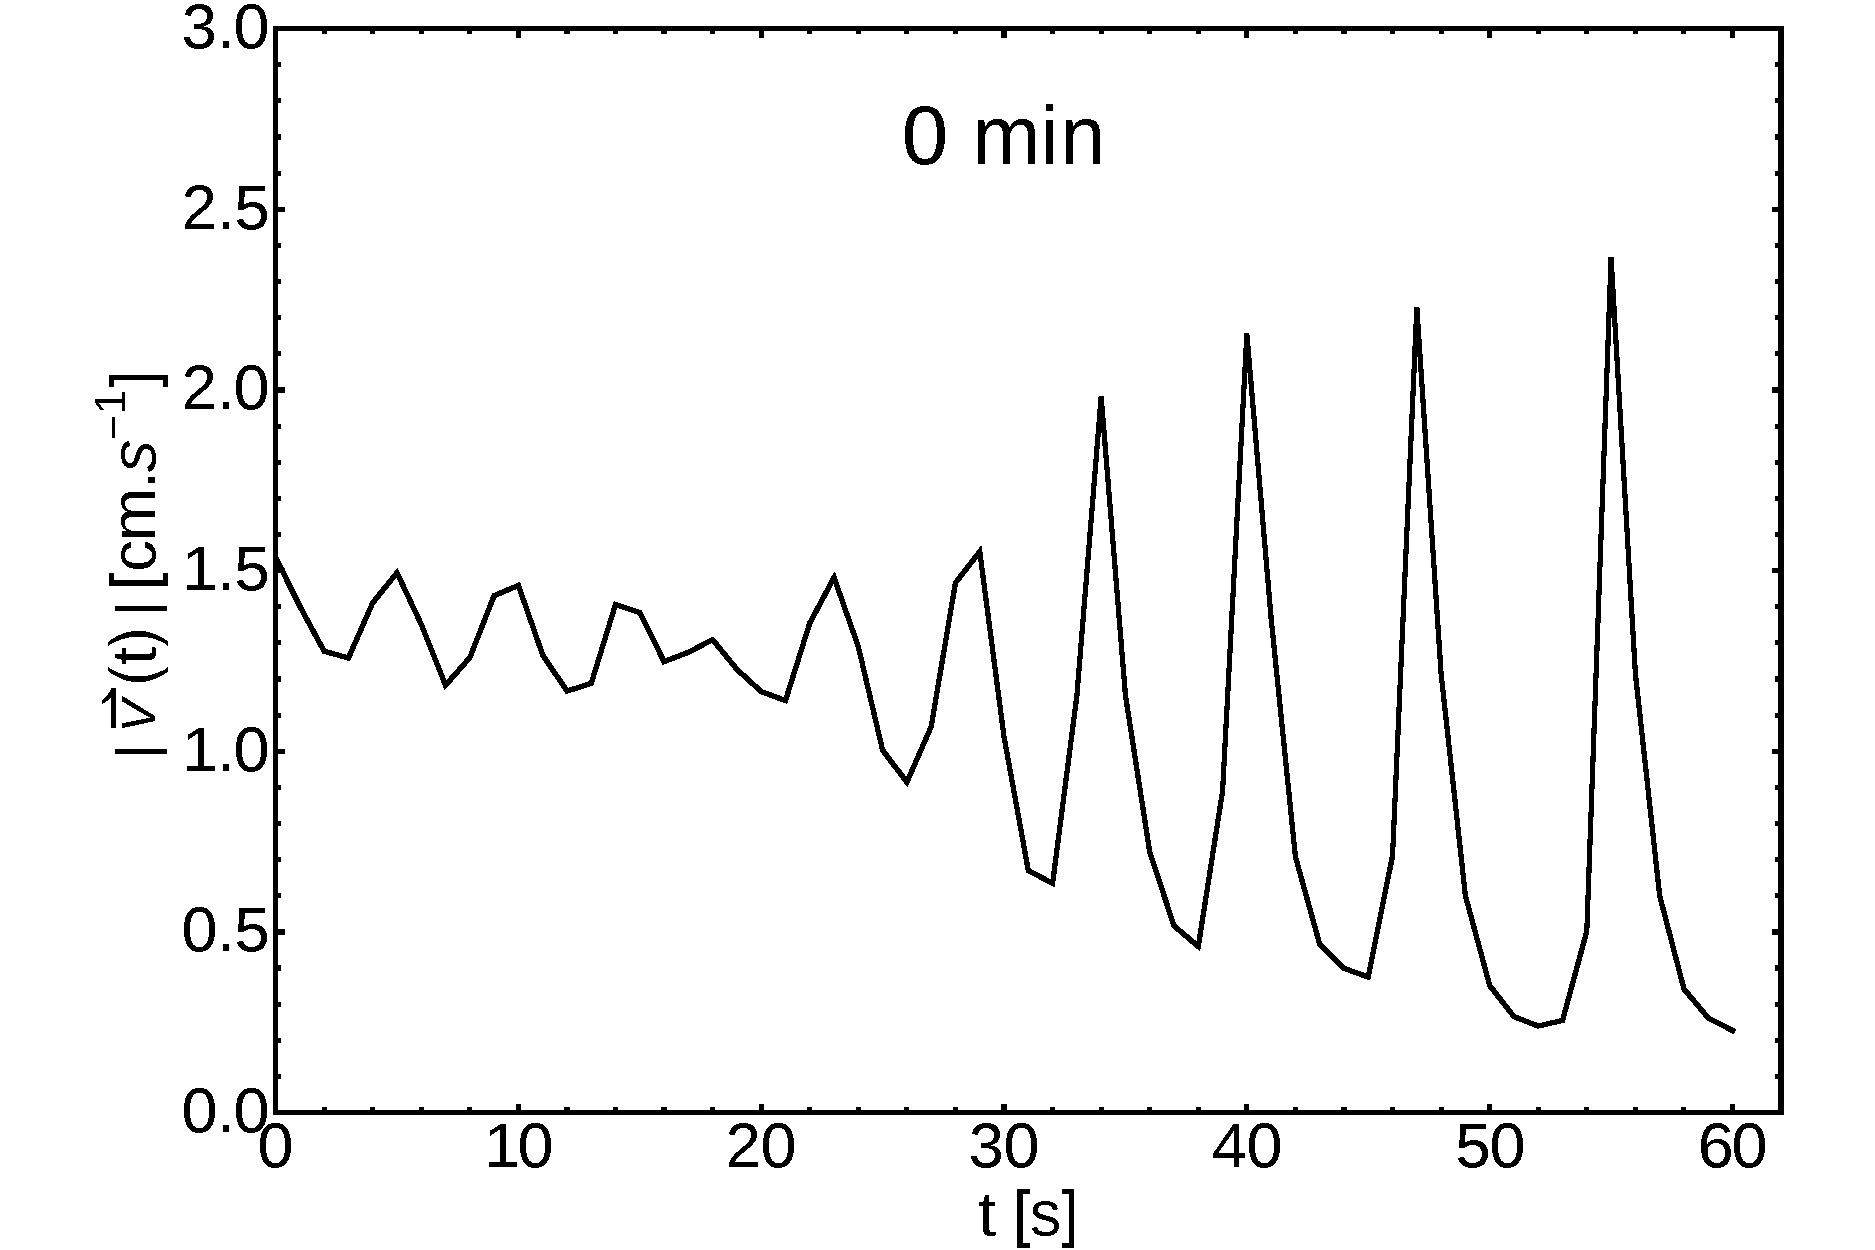
\includegraphics[width=\textwidth]{uvst_65dypcm_a.pdf}
		% \caption{$\xi \simeq \xi_{c}$}\label{fig:uvst_65dypcm_a}		
	\end{minipage}
	\begin{minipage}[c]{0.3\linewidth}
		\centering
		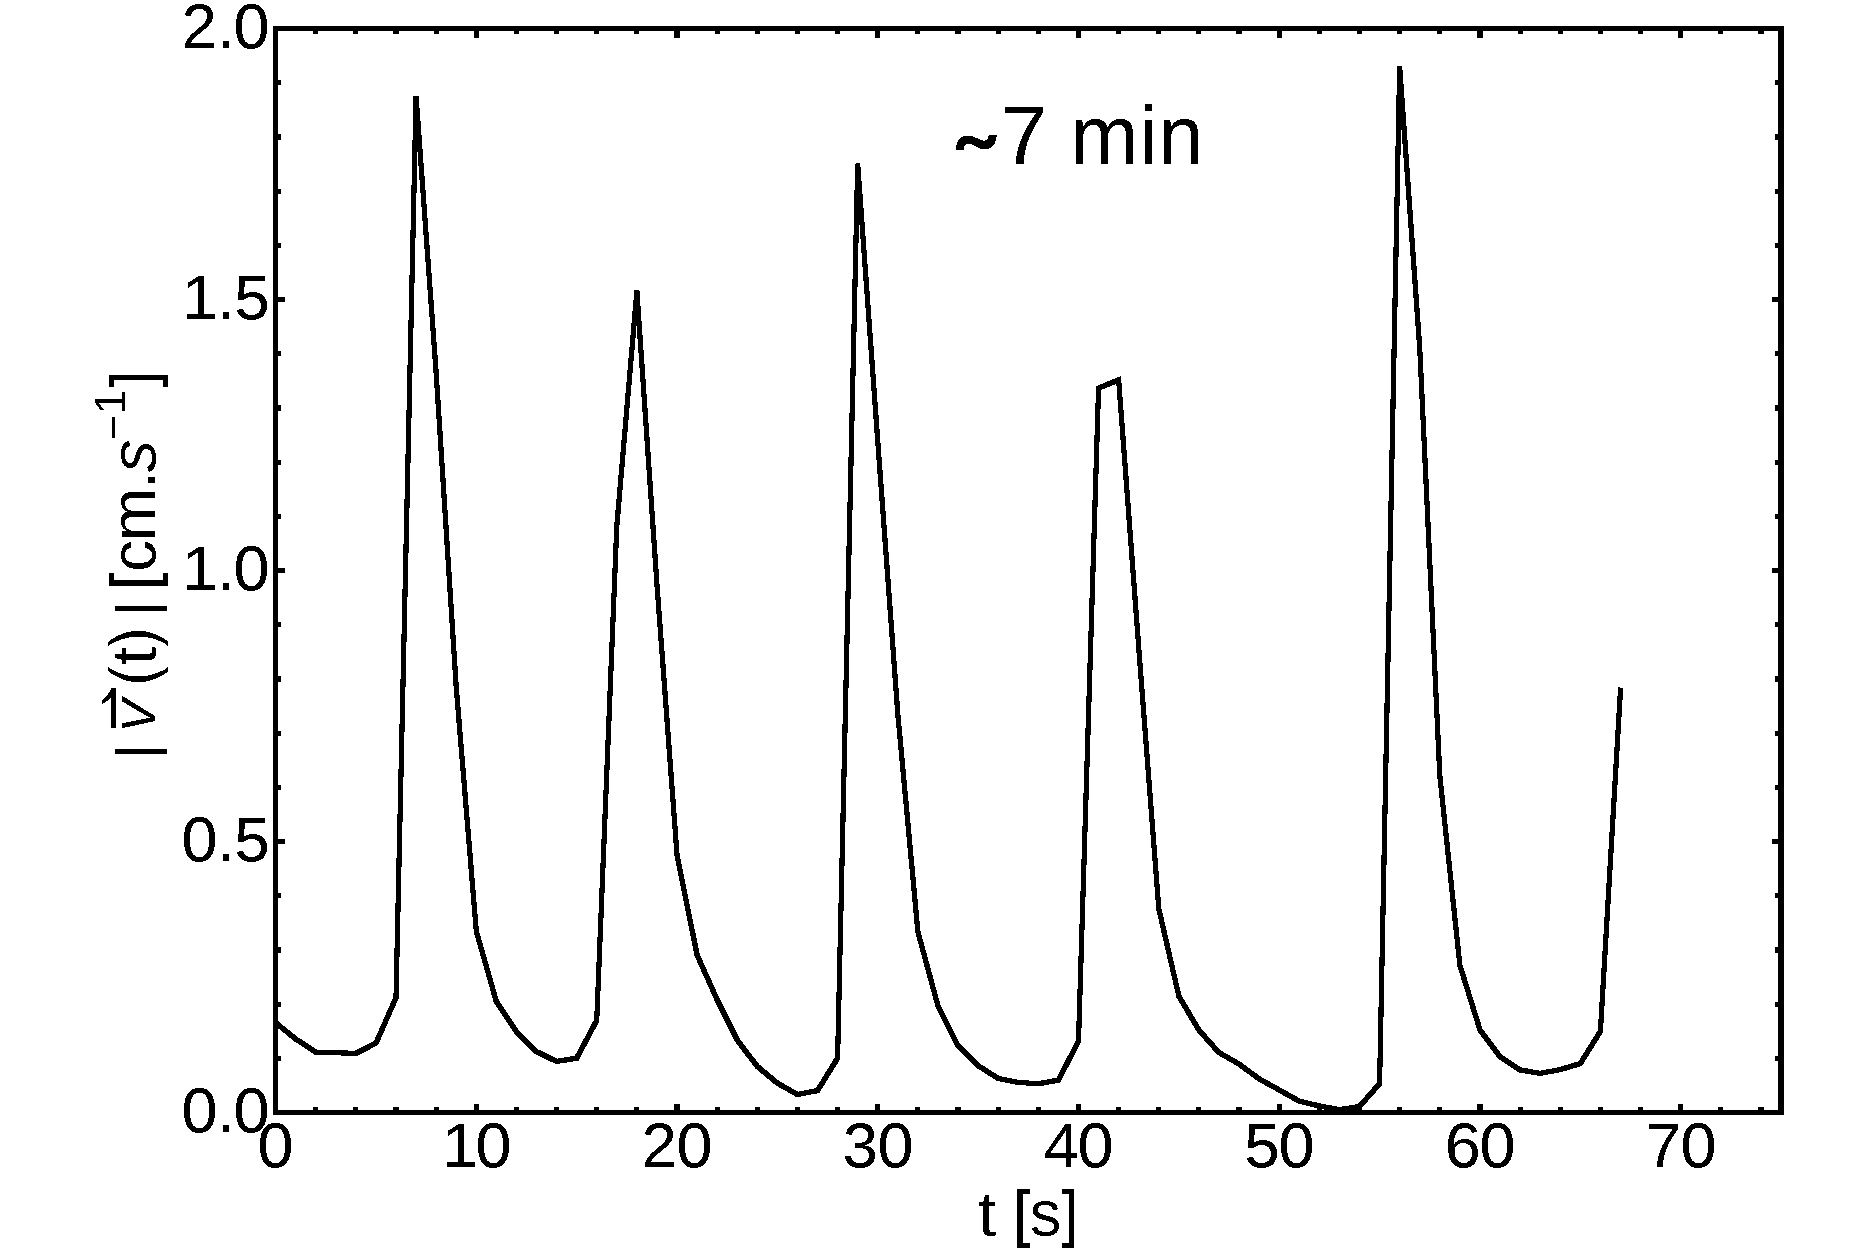
\includegraphics[width=\textwidth]{uvst_65dypcm_b.pdf}
		% \caption{$\xi < \xi_{c}$}\label{fig:uvst_65dypcm_b}
	\end{minipage}
	\begin{minipage}[c]{0.3\linewidth}
		\centering
		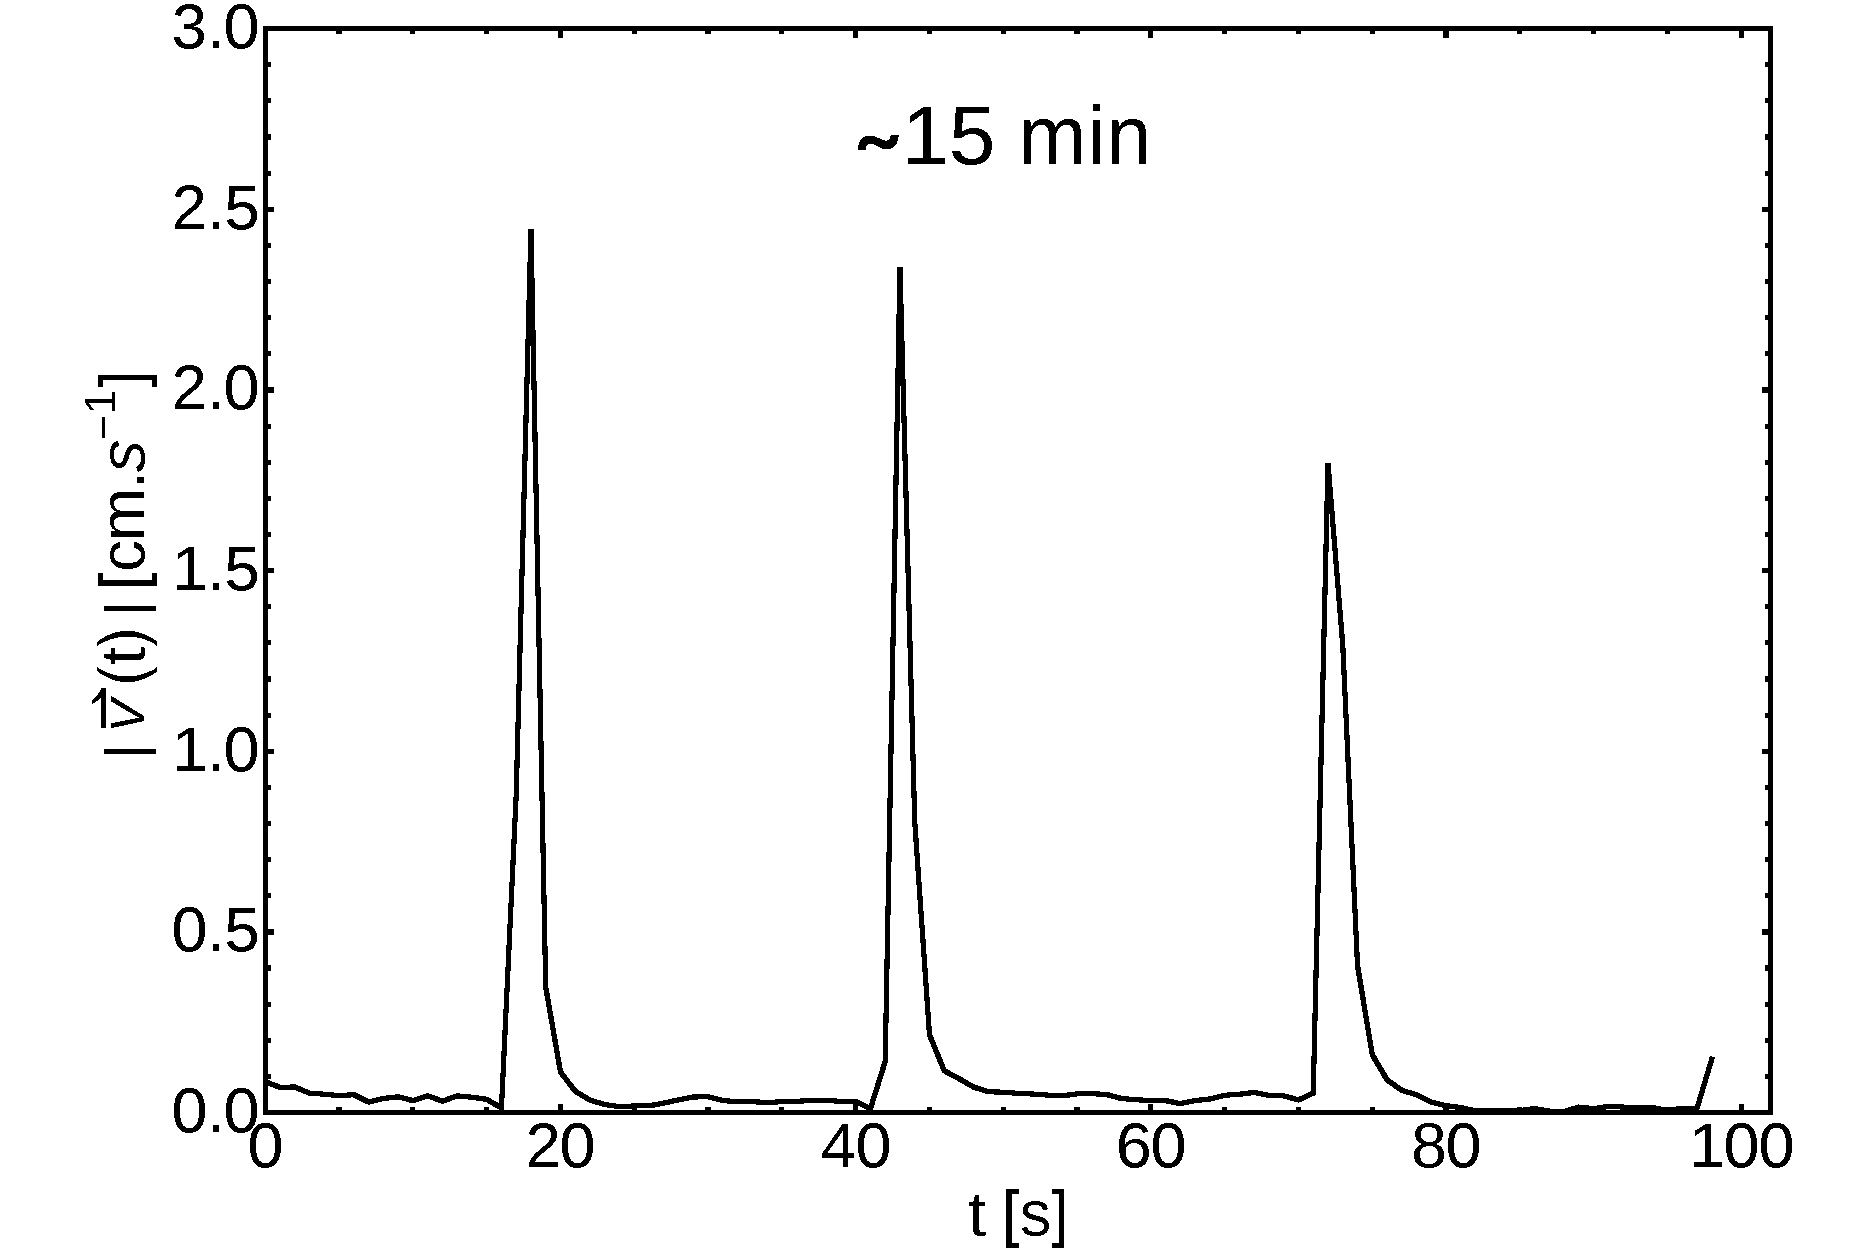
\includegraphics[width=\textwidth]{uvst_65dypcm_c.pdf}
		% \caption{$\xi << \xi_{c}$}\label{fig:uvst_65dypcm_c}
	\end{minipage}
	\caption{$\xi \simeq \xi_{c}$, $\xi < \xi_{c}$ and $\xi << \xi_{c}$}\label{fig:uvst_65dypcm}
\end{figure*}

\begin{figure*}[h!]
    \centering
	\begin{minipage}[t]{0.3\linewidth}
		\centering
		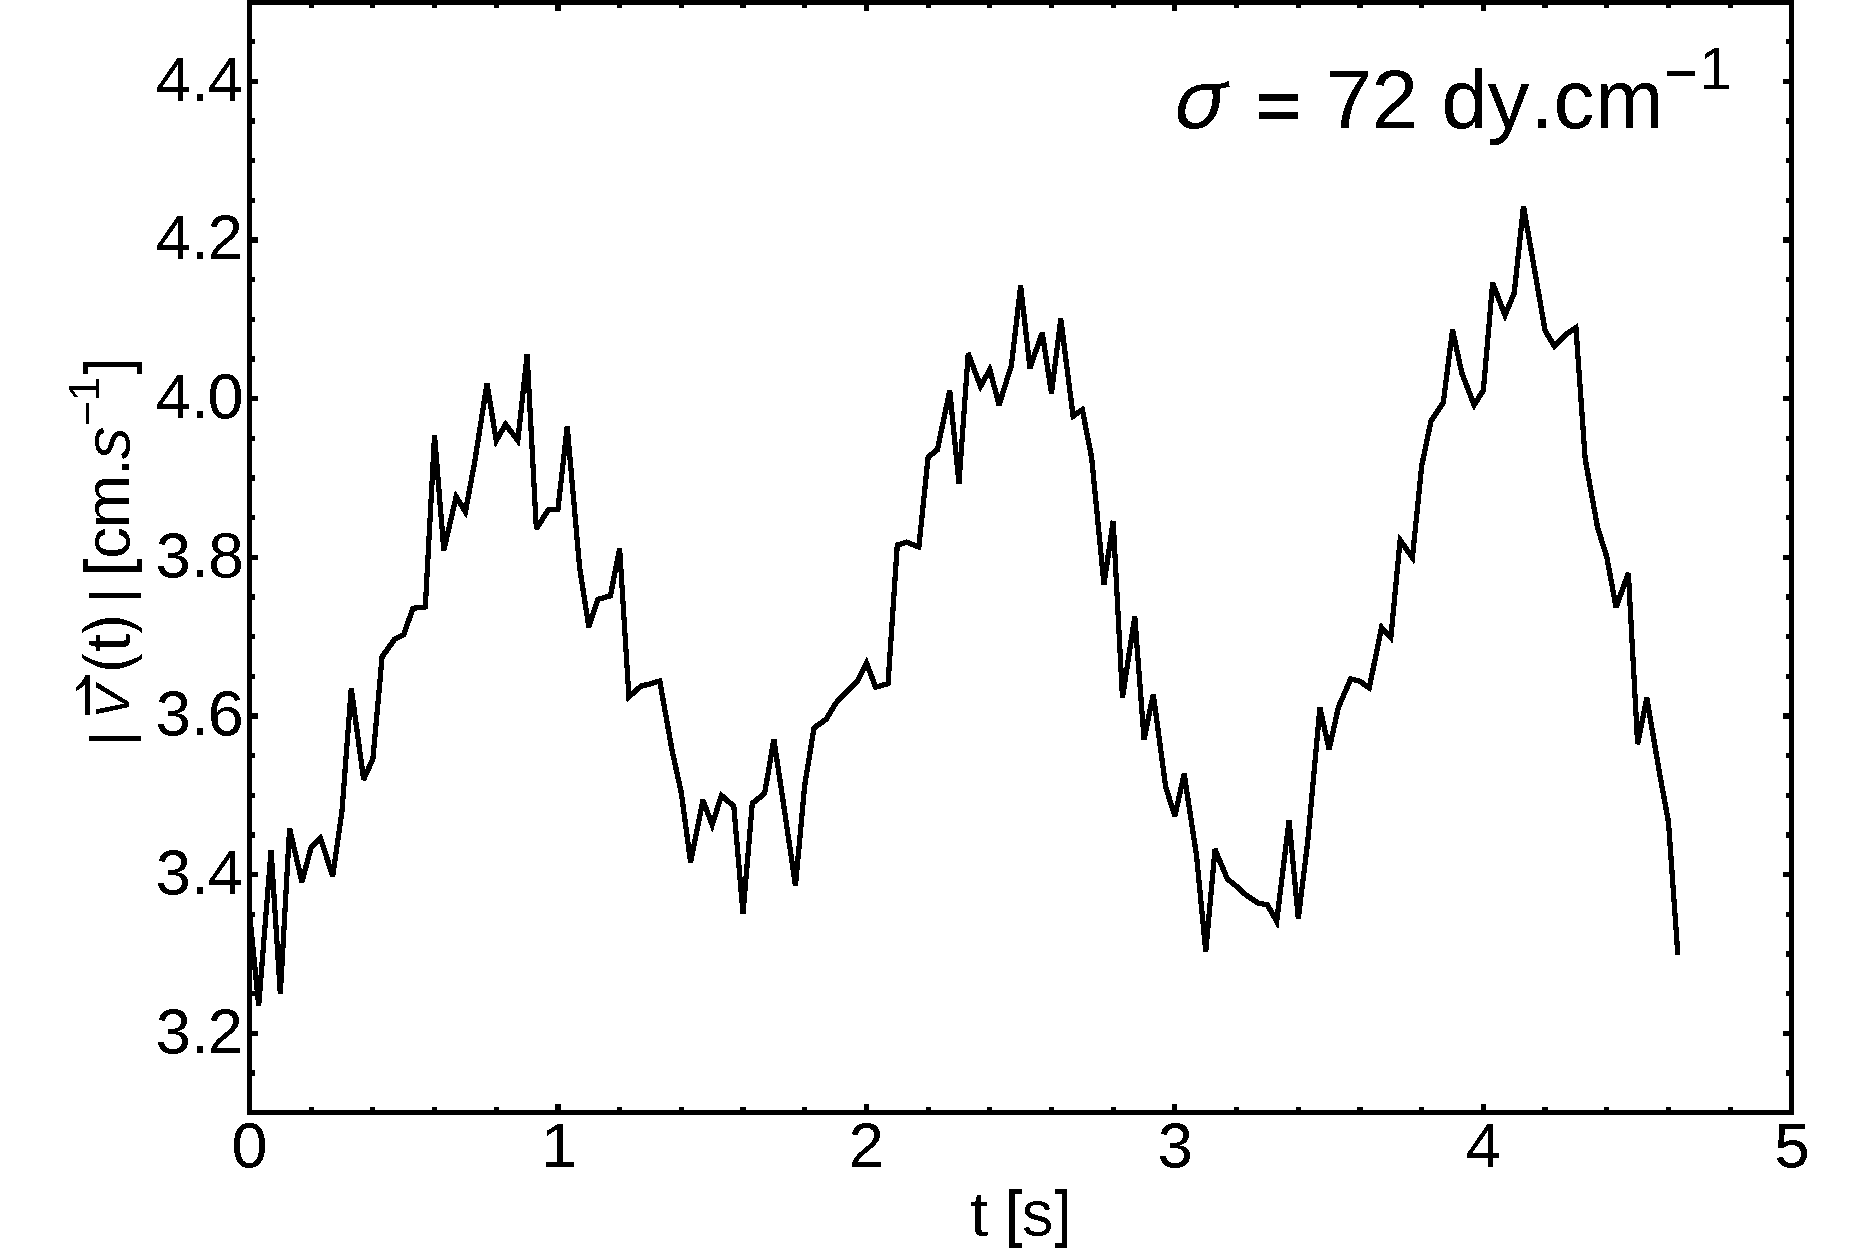
\includegraphics[width=\textwidth]{uvst_sigma_a.pdf}
		% \caption{$\xi > \xi_{c}$}\label{fig:uvst_sigma_a}		
	\end{minipage}
	\begin{minipage}[t]{0.3\linewidth}
		\centering
		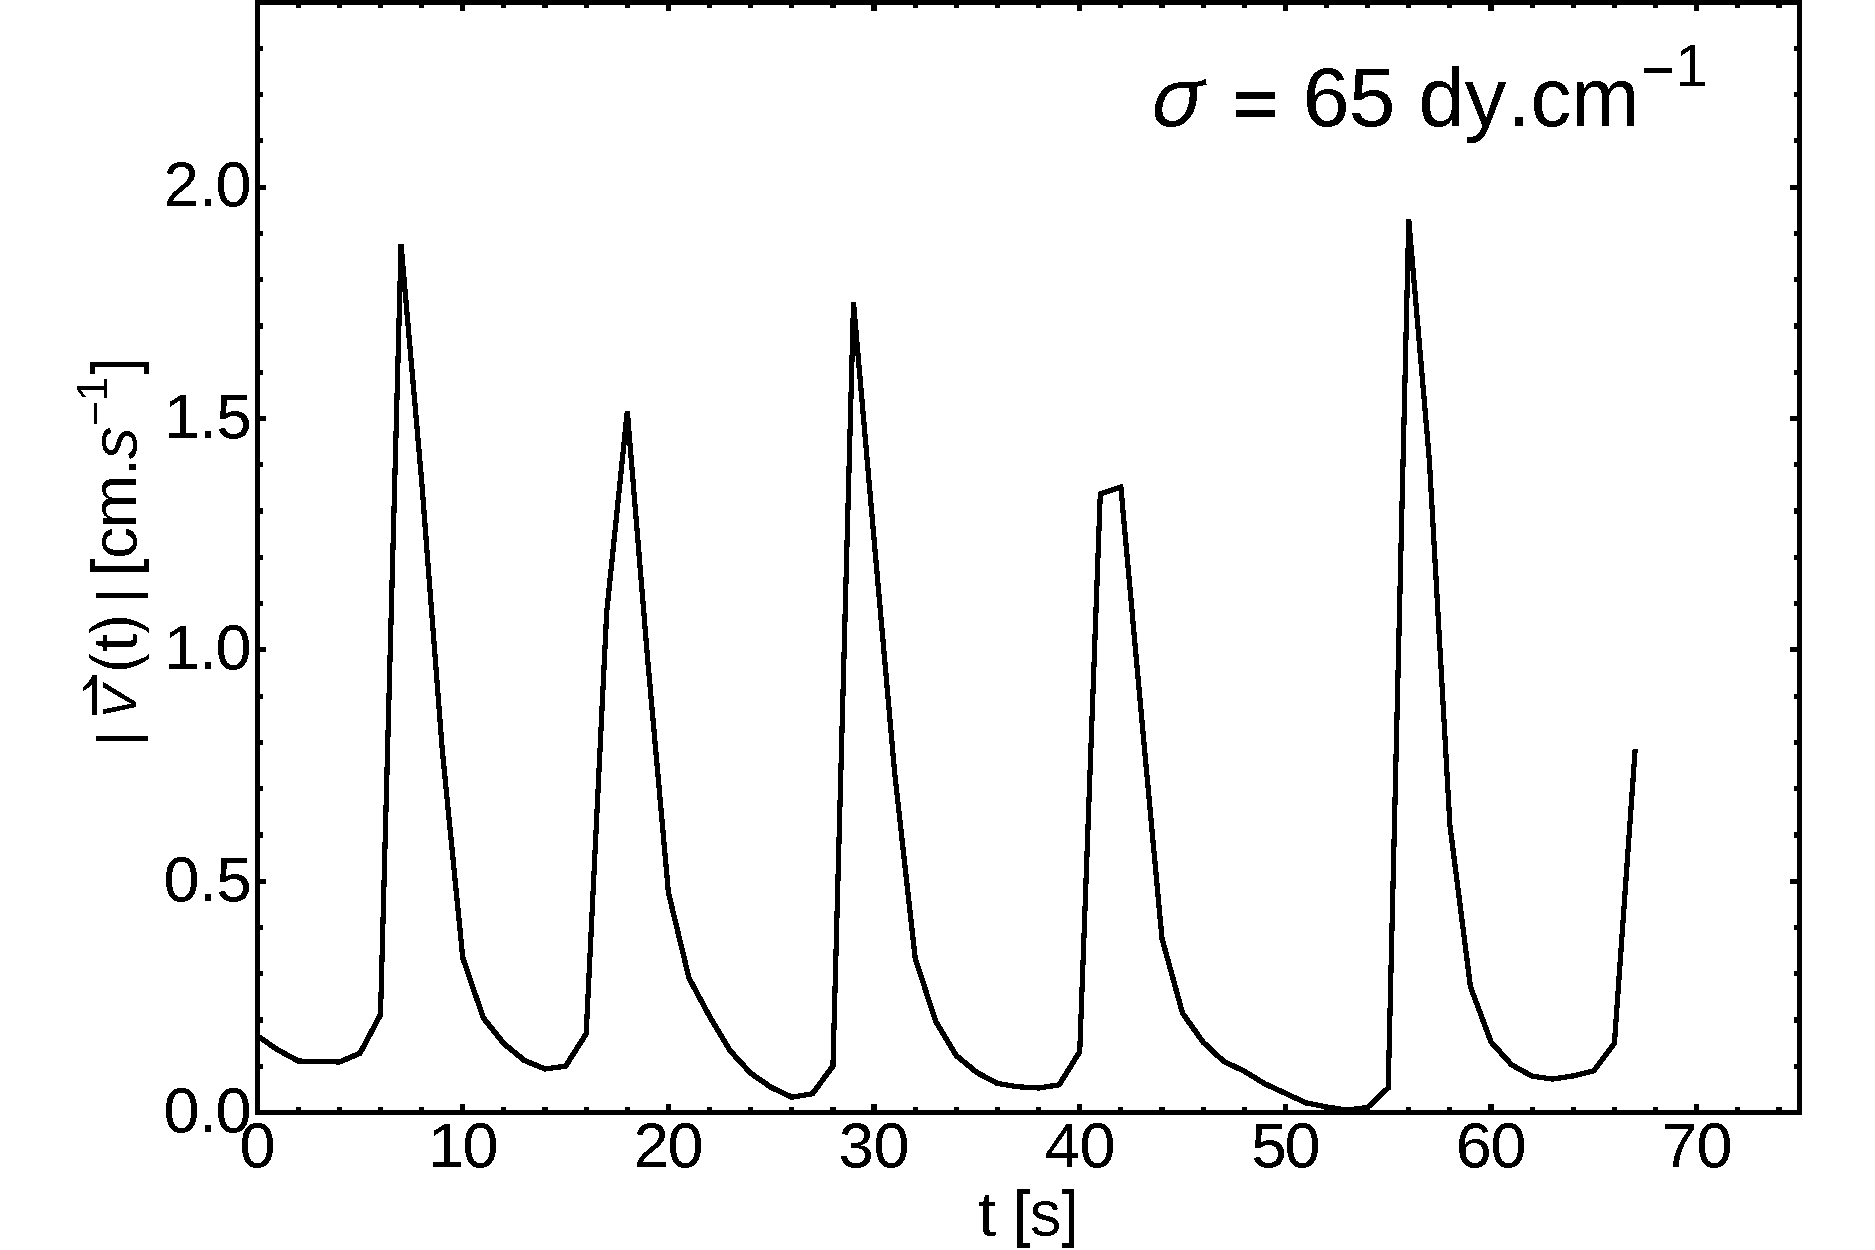
\includegraphics[width=\textwidth]{uvst_sigma_b.pdf}
		% \caption{$\xi \simeq \xi_{c}$}\label{fig:uvst_sigma_b}
	\end{minipage}
	\begin{minipage}[t]{0.3\linewidth}
		\centering
		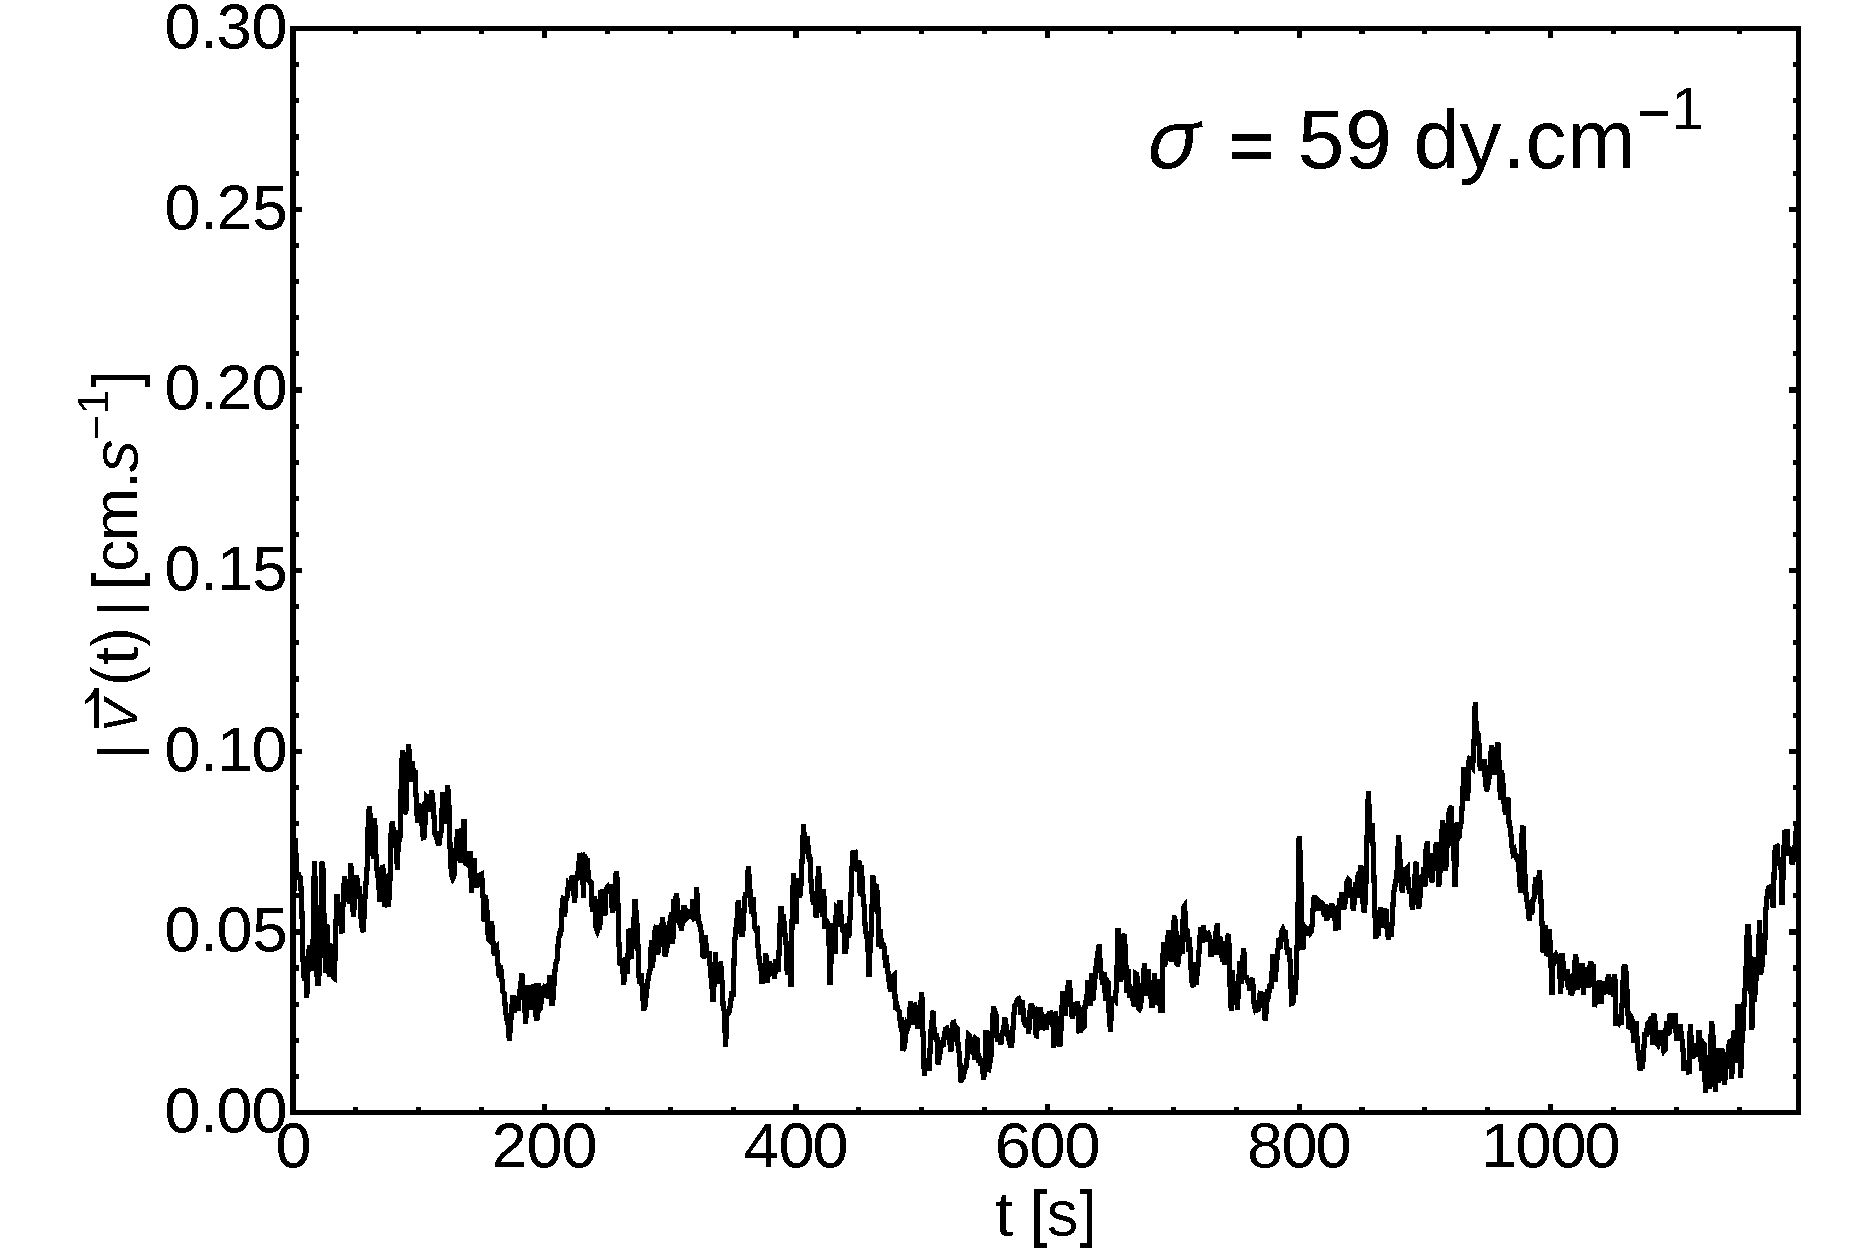
\includegraphics[width=\textwidth]{uvst_sigma_c.pdf}
		% \caption{$\xi < \xi_{c}$}\label{fig:uvst_sigma_c}
	\end{minipage}
	\caption{$\xi > \xi_{c}$, $\xi \simeq \xi_{c}$ and $\xi < \xi_{c}$}\label{fig:uvst_sigma}
\end{figure*}
\section{Summary}
\label{sec:summary}


\acknowledgments
VSA, DKS, and MMB were supported by the OIST Graduate University with subsidy funding from the Cabinet Office, Government of Japan. MMB acknowledges L. Mahadevan for introducing the camphor boat system and subsequent scientific discussions, and D. Vu Anh for help with preliminary experiments.

\bibliography{all}

\end{document} 
